\section{UX Diagrams}
The purpose of this section is to show the possible screens that the user might encounter during the use of the system.
The displayed information and the possible interactions by the user are also shown in these diagrams.\\
To allow a better reading of the diagrams themselves, they have been divided into 4 parts:
\begin{itemize}
  \item Diagram of Data4Help (accessible from Web Wrowser), Figure \ref{img:Data4Help}.
  \item Diagram of Track4Run (accessible from Web Wrowser), Figure \ref{img:Track4RunWeb}.
  \item Diagram of Track4Run (accessible from the App on Smartphone), Figure \ref{img:Track4RunApp}.
  \item Diagram of AutomatedSOS (accessible from the App on Smartphone), Figure \ref{img:AutomatedSOSApp}.
\end{itemize}
The AutomatedSOS diagram contains a screen unreachable by the user. It is the screen that is displayed when an emergency is detected and then an ambulance is alerted. For this screen to be displayed, the user must be logged in to the app and have connected a device.

\begin{figure}[H]
  \begin{center}
  	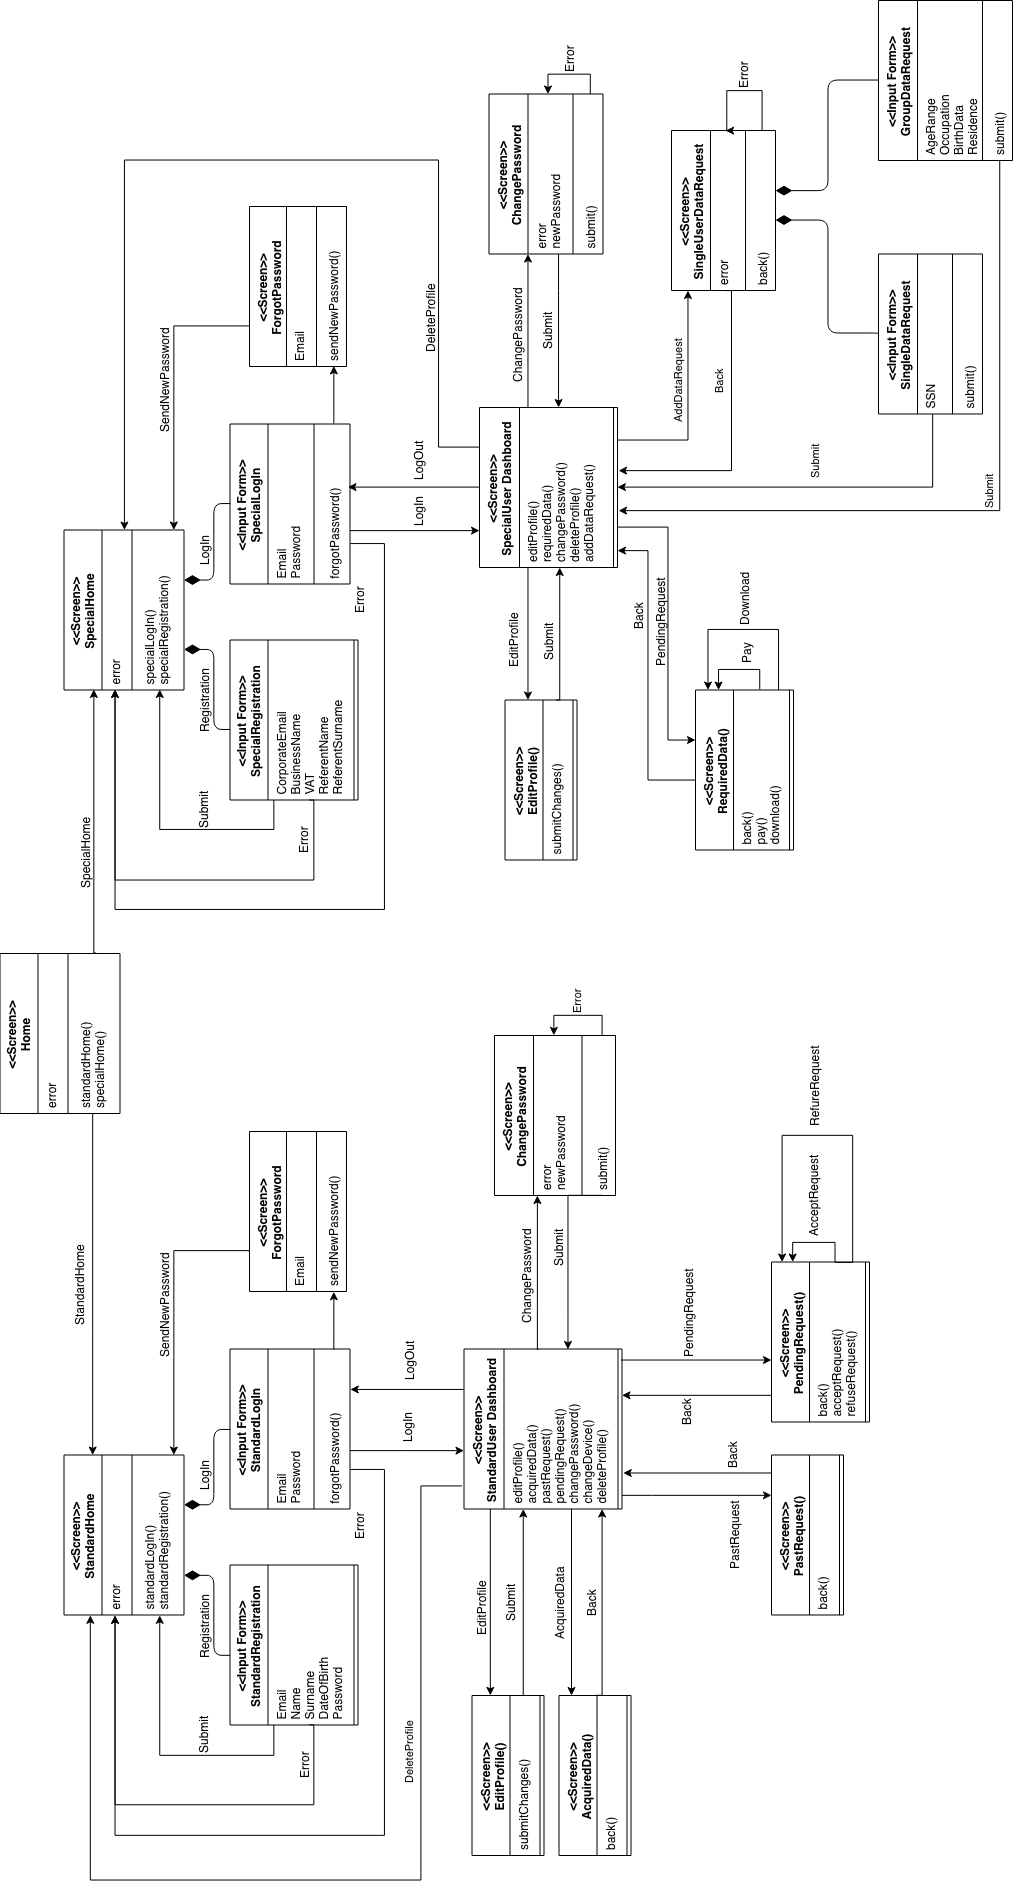
\includegraphics[height=0.68\paperheight]{./img/UXDiagram/UX_Diagram_Data4Help.png}
    \hspace{0.05\linewidth}
    \centering
    \caption{UX Diagram \textit{Data4Help} (Web)}
		\label{img:Data4Help}
    \end{center}
\end{figure}

\begin{figure}[H]
  \begin{center}
  	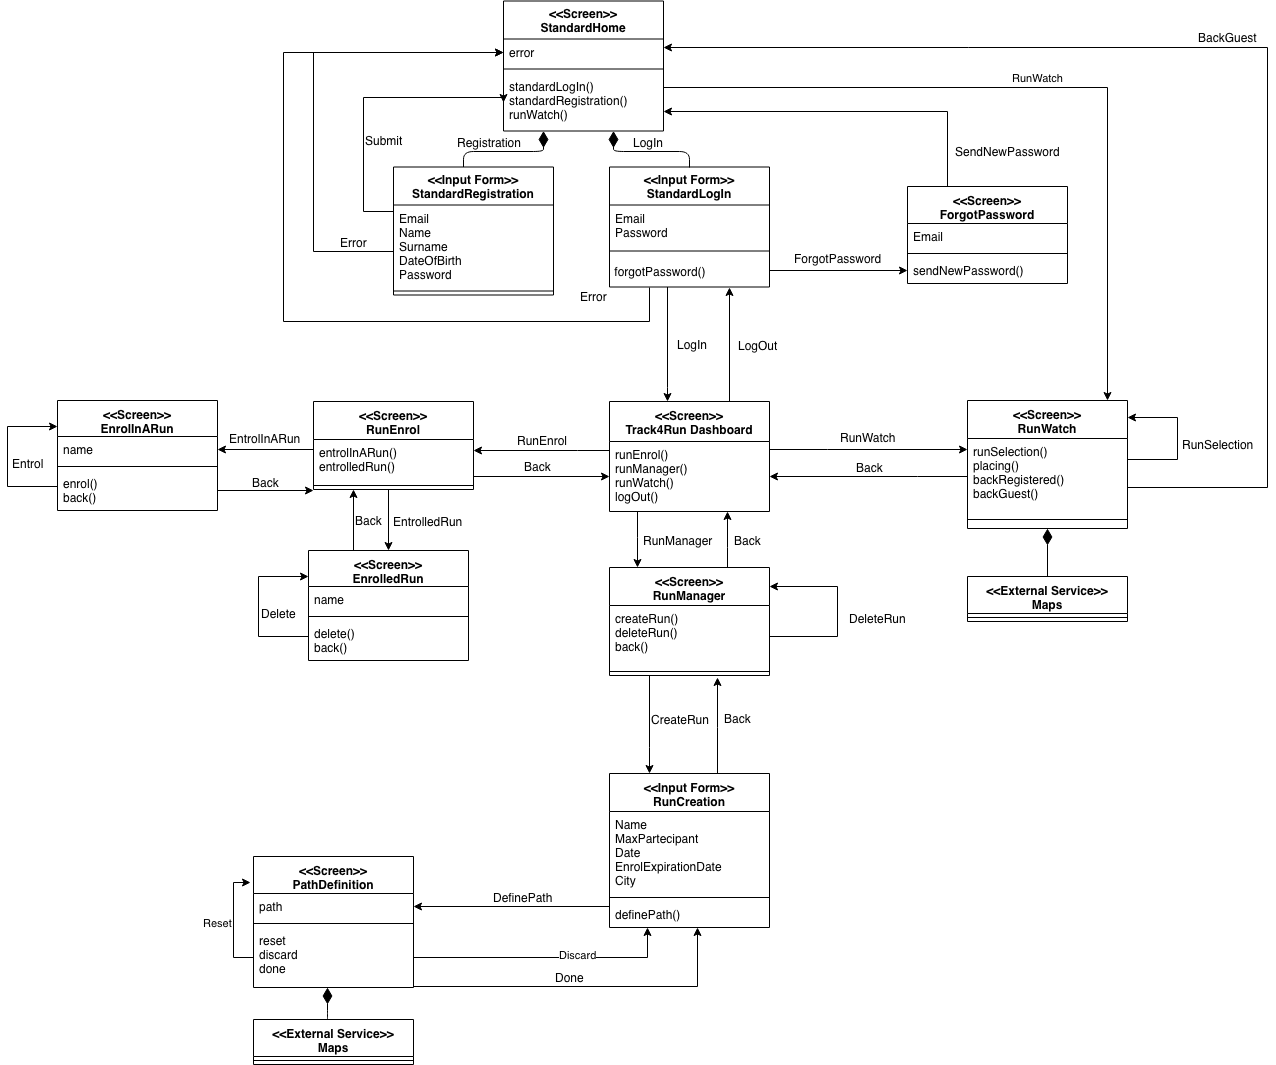
\includegraphics[width=0.68\paperwidth]{./img/UXDiagram/UX_Diagram_Track4Run_Web.png}
    \hspace{0.05\linewidth}
    \centering
    \caption{UX Diagram \textit{Track4Run} (Web)}
		\label{img:Track4RunWeb}
    \end{center}
\end{figure}

\begin{figure}[H]
  \begin{center}
  	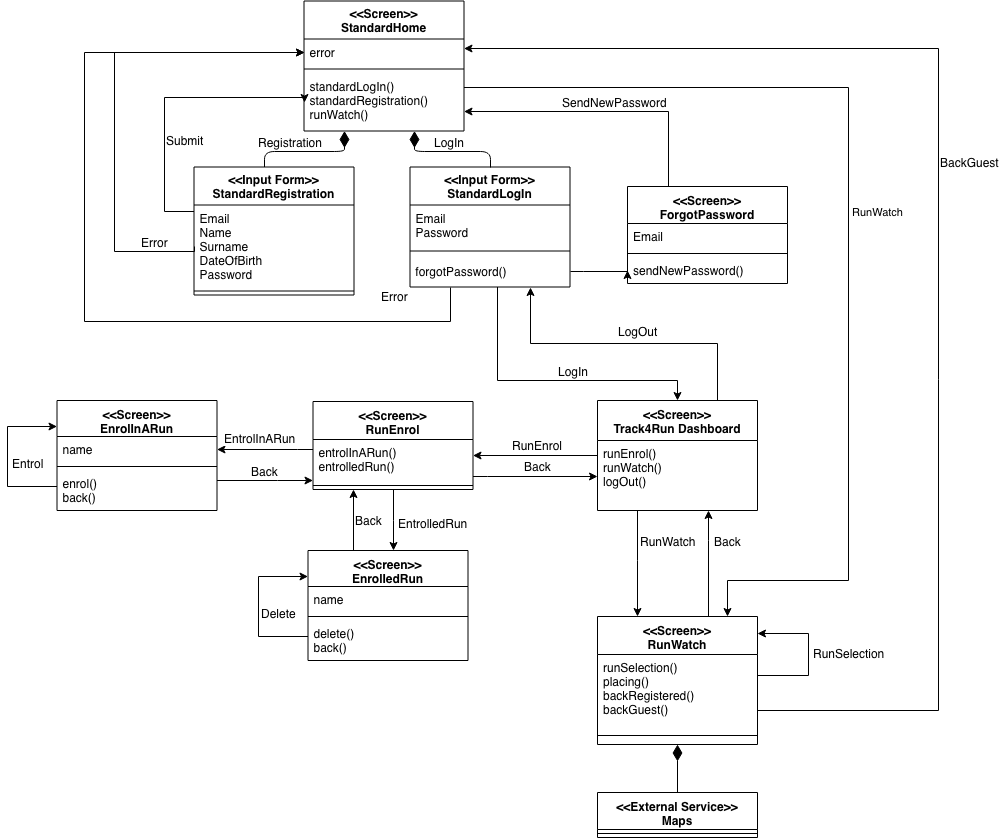
\includegraphics[width=0.68\paperwidth]{./img/UXDiagram/UX_Diagram_Track4Run_App.png}
    \hspace{0.05\linewidth}
    \centering
    \caption{UX Diagram \textit{Track4Run} (App)}
		\label{img:Track4RunApp}
    \end{center}
\end{figure}

\begin{figure}[H]
  \begin{center}
  	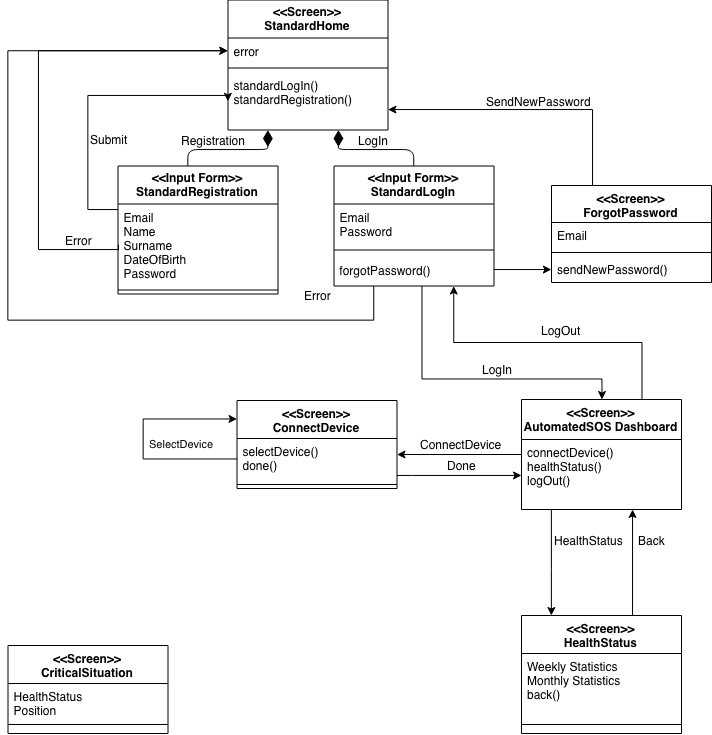
\includegraphics[width=0.68\paperwidth]{./img/UXDiagram/UX_Diagram_AutomatedSOS_App.png}
    \hspace{0.05\linewidth}
    \centering
    \caption{UX Diagram \textit{AutomatedSOS} (App)}
		\label{img:AutomatedSOSApp}
    \end{center}
\end{figure}

\section{User Interfaces}
For user interfaces, please refer to the Requirements Analysis and Specification Document where the mockups have been included and explained.
